\section{Introduction}
This section presents the high level overview of the Occupancy Analyzer system.

\section{System Overview}
The Figure 3.1 (and 3.2) displays different components in the system and how they relate and communicate with each other.

% Tomas' system overview.
\begin{figure}[ht]
	\begin{center}
	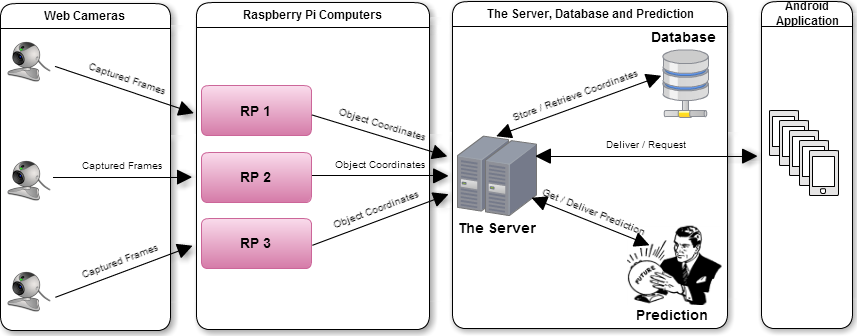
\includegraphics[scale=0.54]{system_overview/system_overview_tomas}
	\caption{Occupancy Analyzer System Overview}
	\end{center}
\end{figure}

% Theresa's system overview.
\begin{figure}[ht]
	\begin{center}
	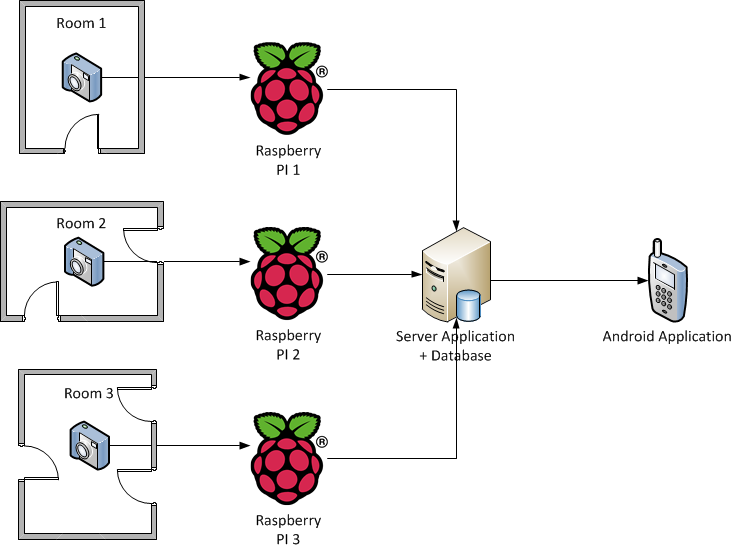
\includegraphics[scale=0.54]{system_overview/system_overview_theresa}
	\caption{System overview of the occupancy analyzer}
	\end{center}
\end{figure}

As we can see, the system primarily consists of 4 components:

\begin{enumerate}
	\item Web Cameras;
	\item Raspberry Pi Computers;
	\item The Server;
	\item and The Android Application.
\end{enumerate}

All of these components are discussed further on in the respected chapters.

%camera placement and positioning reference: http://www.lorextechnology.com/support/self-serve/Camera-Location-Placement-and-Positioning/2700036
\section{Web Cameras}
The purpose of the web cameras is simply to surveillance the area they have been placed in and forward the captured frames to Raspberry Pi computers for further processing, as shown in Figure 3.1 (and 3.2). The cameras can be placed in a room, corridor, atrium or any other similar place in or outside the building, where people detection and their movement prediction is required. Camera can either be placed directly above the observed area or in the corner of it as illustrated in Figure 3.3. Naturally, a camera placed above the observed area would give better results, since this increases it's field of view, as well as makes it easier to correctly detect and distinguish between multiple people walking side by side. Furthermore, for the best results one must also take many different factors into account, such as
the distance between the camera and monitored area, environmental conditions of the area the camera is placed in, lighting conditions, and many others.

% Camera placement images.
\begin{figure}[ht]
	\begin{center}
	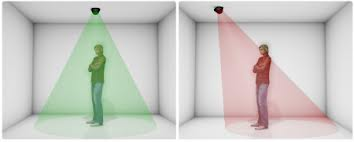
\includegraphics[scale=0.65]{camera_placement/camera_placement_1}
	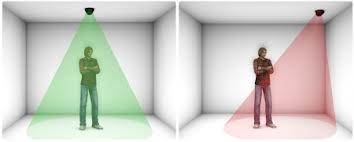
\includegraphics[scale=0.65]{camera_placement/camera_placement_2}
	\caption{Camera placement in a room}
	\end{center}
\end{figure}

\section{Raspberry Pi Computers}
The next component in the system architecture is Raspberry Pi computers. These computers have at least one web camera attached to them, and are responsible for processing the frames captured by that camera. The main goal of processing these frames is to try to detect people in the monitored area and determine their position in that area. There are many different challenges in object detection, as well as various concepts and techniques that can be used to achieve this, thus we discuss them in the next chapter.
	
	\subsection{Object Extraction}
	To detect and extract objects, or in our case, people and their movement, we need to apply several motion detection techniques on the frames we are receiving from the web camera. First of all, to detect changes in some monitored area, we naturally need to have at minimum two images, which we must compare to see what changes occurred. We will try to look into two different approaches in doing this, a simple one, but at the same time less flexible, and a bit more complicated and sophisticated approach, but much more adaptive and flexible.
	
	% Background subtraction reference: http://profs.sci.univr.it/~cristanm/teaching/sar_files/lezione4/Piccardi.pdf
	\subsubsection{Background Subtraction Approach}
	To begin with, a simple approach, called Background Subtraction, would be to have a one static background image of observed area that was taken prior and did not have any people in it. Then, one can simply detect changes and movement in the area by subtracting the static background image from every newly taken image of the monitored area at some given rate, for example taking a new image of the area every 2 seconds. The difference between the two images would then allow us to see if any changes happened, since after subtraction the resulting image would either be totally black (Figure 3.4), meaning no one walked passed the observed area, or the image would have some resulting bright contours of detected object or objects (Figure 3.5).
	% Background Subtraction with no background changes.
	\begin{figure}[ht]
		\begin{center}
		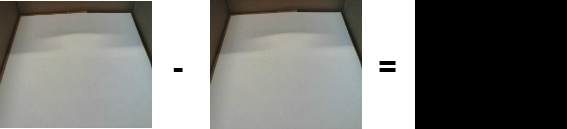
\includegraphics[scale=0.65]{background_subtraction/background_subtraction_1}
		\caption{Background Subtraction with no background changes}
		\end{center}
	\end{figure}
	% Background subtraction with background changes (lego man appearing).
	\begin{figure}[ht]
		\begin{center}
		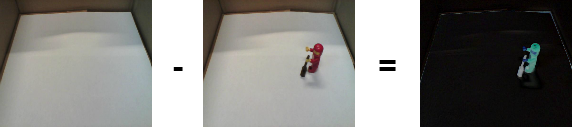
\includegraphics[scale=0.65]{background_subtraction/background_subtraction_2}
		\caption{Background Subtraction with background change}
		\end{center}
	\end{figure}
	\\After doing some research and experimenting with background subtraction technique, one will quickly discover that there are multiple weaknesses to it. First of all, if the initial background image is always static and never changes, this technique will fail in environments where lighting is dynamic. This is perfectly illustrated in Figure 3.6. We can see that the lighting is much darker in the second image, possibly because the light was turned off in the monitored room, thus after subtracting our static background image from this image, the resulting image is simply a lighter version of the two images, and not the intended black image. This is a big problem, because now even if a person moves through the monitored area, he or she will not be easily extracted as in Figure 3.5, since the whole background of the newly taken image is interpreted as a totally different background than the original static background and will appear in the resulting image. This is illustrated in Figure 3.7. 
	% Background subtraction with background changes (lighting changes).
	\begin{figure}[ht]
		\begin{center}
		
\includegraphics[scale=0.65]{background_subtraction/background_subtraction_3}
		\caption{Background Subtraction with background lighting change}
		\end{center}
	\end{figure}
	% Background subtraction with background changes (lighting changes + lego figure).
	\begin{figure}[ht]
		\begin{center}
		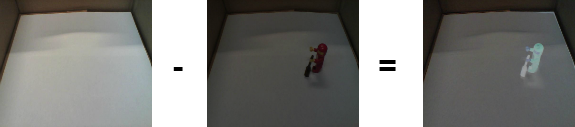
\includegraphics[scale=0.65]{background_subtraction/background_subtraction_4}
		\caption{Background Subtraction with background lighting change and lego figure appearing}
		\end{center}
	\end{figure}
	\\Another problem with background subtraction approach is that if a camera is placed inside an area which has objects that constantly change their original position (chairs, tables, appliances, etc.) by being moved, even small changes in object's location will spoil the resulting image after subtraction. As we can see in Figure 3.8, the object is displayed twice in the resulting image, even thought we were not even interested in it, making it much harder to detect actual people moving in the area. From now on, the resulting image after subtraction will always be corrupt unless the object is placed back to it's original position.
		% Background subtraction with background changes (object changes location).
	\begin{figure}[ht]
		\begin{center}
		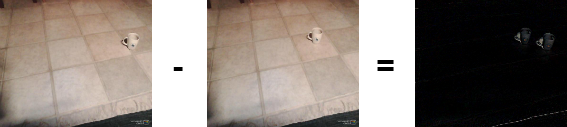
\includegraphics[scale=0.65]{background_subtraction/background_subtraction_5}
		\caption{Background Subtraction with object changing it's location}
		\end{center}
	\end{figure}
	\\In conclusion, we can see that background subtraction approach can work well in static environments, however it falls short in dynamic spaces. Naturally, these mentioned drawbacks of background subtraction approach need to be handled for object detection to work well, which unnecessarily creates additional challenges when implementing the system.
	% Moving Average references: http://derek.simkowiak.net/motion-tracking-with-python/, http://opencvpython.blogspot.dk/2012/07/background-extraction-using-running.html
	\subsubsection{Moving Average Approach}
	A much better and preferred approach for movement detection is using moving average method. In this technique we do not need to rely on a static background image of the monitored area taken prior. Instead, we try to find a new "approximate" background image by interpreting any changes in the background as noise and blurring them out. This exact approach is illustrated in figures 3.9 and 3.10. As we can see, hand motion moving up and down gets blurred out when applying moving average method, thus producing an approximate background image that can be used for subtraction of the original frame from it. After subtraction, the motion areas will simply stand out against a black background of non-motion, as it was similarly shown in Figure 3.5. This method of object extraction works very well and has a lot of flexibility, since it can adapt to environmental changes in monitored area, thus eliminating most of the weaknesses that background subtraction approach has. For these reasons, moving average approach was chosen for our design.
	% Moving average 1.
	\begin{figure}[ht]
		% minipage allows to put 2 figures in one line.
		\begin{minipage}[b]{0.50 \linewidth}
		\centering
		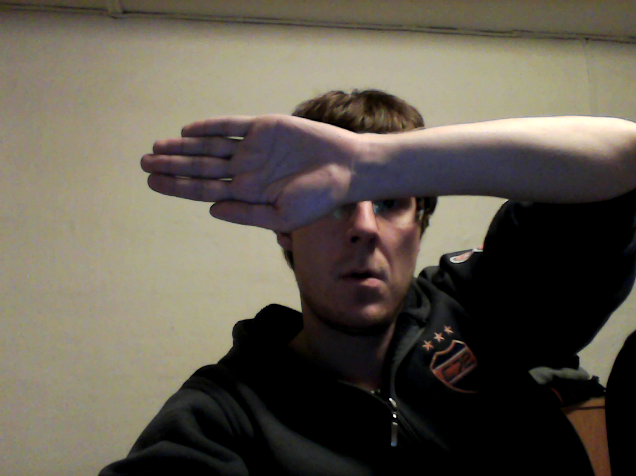
\includegraphics[scale=0.30]{moving_average/moving_average_1}
		\caption{Original frame}
		\end{minipage}
		\begin{minipage}[b]{0.50 \linewidth}
		\centering
		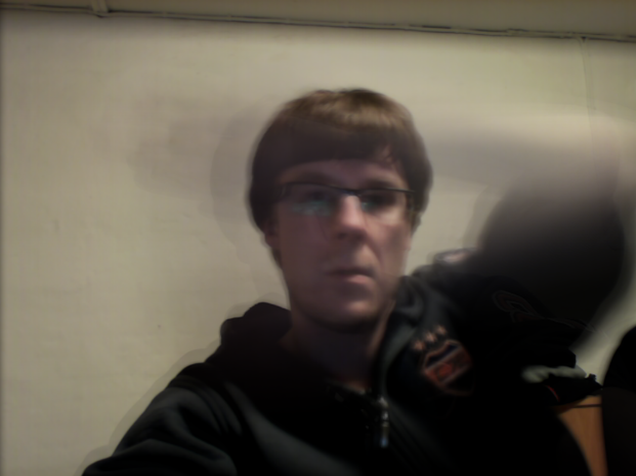
\includegraphics[scale=0.30]{moving_average/moving_average_2}
		\caption{Moving average frame}
		\end{minipage}
	\end{figure}
	
	\subsection{Object Detection}
	Now that we can extract objects using moving average technique, we need to be able to actually find them in the resulting image we get after we perform subtraction. For this, we need to apply several key techniques in image processing. \\If we start at the beginning, after we capture the initial frame of the monitored area, it will often contain noise and small details that we are not interested in. To deal with this, we must first apply blur or smoothing filter, which helps to reduce image noise and detail, as shown in figures 3.10 and 3.11.
	% Blur example.
	\begin{figure}[ht]
		% minipage allows to put 2 figures in one line.
		\begin{minipage}[b]{0.50 \linewidth}
		\centering
		
\includegraphics[scale=0.30]{blur/blur_1}
		\caption{Original frame}
		\end{minipage}
		\begin{minipage}[b]{0.50 \linewidth}
		\centering
		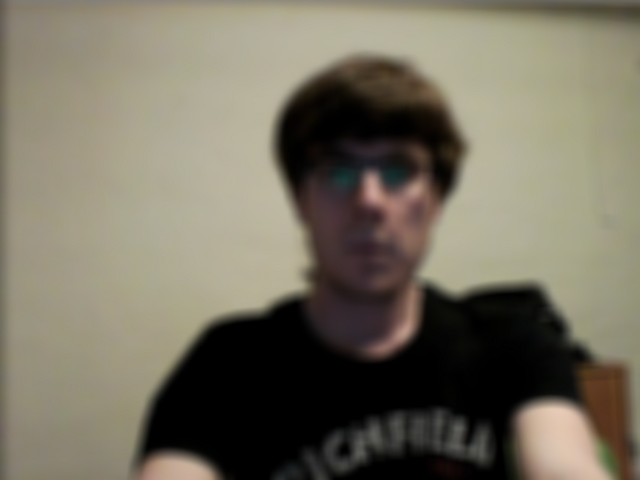
\includegraphics[scale=0.30]{blur/blur_2}
		\caption{Frame after blur is applied}
		\end{minipage}
	\end{figure}
	% Reference for grayscale channel #: http://docs.gimp.org/en/gimp-images-in.html
	% Reference for erosion: http://homepages.inf.ed.ac.uk/rbf/HIPR2/erode.htm
	\\After we remove the initial noise, we can perform subtraction using moving average approach (described in section 3.4.1.2). After subtraction we will either get a totally black image, meaning no motion occurred, or an image where some colors stand out, meaning some motion has occurred. In either case, for further processing of the taken frame, we need to convert it to a grayscale image. The reason for this is that the original RGB image we get has three channels, while grayscale image has only one, thus it is easier to work with. This procedure is illustrated in figures 3.13, 3.14 and 3.15. \\For further processing of the image, we apply threshold technique, which converts the image to black and white and removes some more unwanted details and noise. After threshold is applied we get the image shown in Figure 3.16. \\Moreover we want to expand the interesting parts of the image and contract smaller pieces, which can be consider noise and managed to slip through, even after we performed thresholding. To do so, we use two fundamental operations in morphological image processing, that is, dilation and erosion. Dilation allows us to probe and expand the shapes contained in the image, whereas erosion simply shrinks shapes, so that bright regions surrounded by dark regions shrink in size, and dark regions surrounded by bright regions grow in size. When we apply dilation and erosion we get the image shown in Figure 3.17. \\Now, to project the detected area onto the original frame, we simply use bounding box technique, which gives us the coordinates of the rectangular border that fully covers the extracted white silhouette that we got in Figure 3.17. Then we use these coordinates to draw a simple rectangular, as well as mark it's middle position by a red circle, as illustrated in Figure 3.18.
	% Grayscale example + threshold.
	\begin{figure}[ht]
		% minipage allows to put 2 figures in one line.
		\begin{minipage}[b]{0.50 \linewidth}
		\centering
		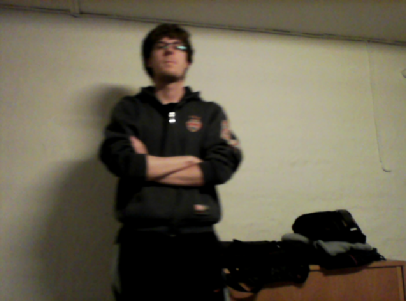
\includegraphics[scale=0.50]{grayscale/grayscale_1}
		\caption{Original frame}
		\end{minipage}
		\begin{minipage}[b]{0.50 \linewidth}
		\centering
		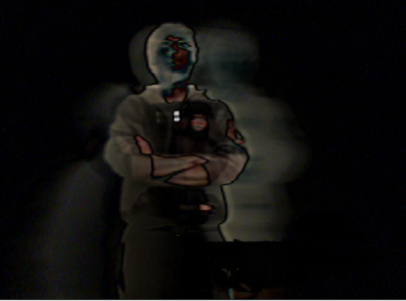
\includegraphics[scale=0.50]{grayscale/grayscale_2}
		\caption{After subtraction}
		\end{minipage}
		\begin{minipage}[b]{0.50 \linewidth}
		\centering
		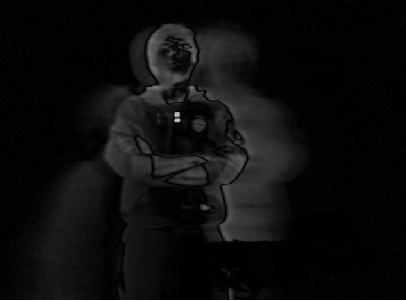
\includegraphics[scale=0.50]{grayscale/grayscale_3}
		\caption{After grayscale filter is applied}
		\end{minipage}
		\begin{minipage}[b]{0.50 \linewidth}
		\centering
		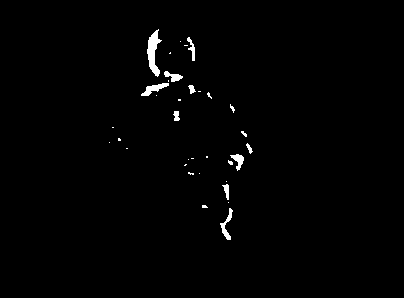
\includegraphics[scale=0.50]{threshold/threshold_1}
		\caption{After threshold is applied}
		\end{minipage}
		\begin{minipage}[b]{0.50 \linewidth}
		\centering
		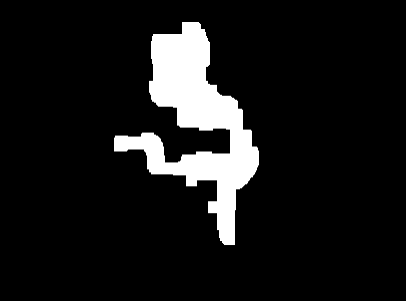
\includegraphics[scale=0.50]{dilate_erode/dilate_erode_1}
		\caption{After dilation and erosion}
		\end{minipage}
		\begin{minipage}[b]{0.50 \linewidth}
		\centering
		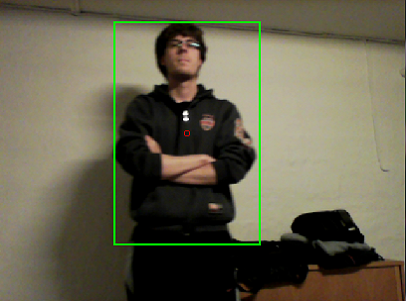
\includegraphics[scale=0.50]{bounding_box/bounding_box_1}
		\caption{After bounding box is drawn}
		\end{minipage}
	\end{figure}
	\\In conclusion, by applying the steps discussed in this section, we can fairly accurately detect people and their movement in the monitored area.
	
	\subsection{Object Differentiation}
	There will naturally be cases when multiple people will walk through monitored area and will be captured by the cameras, therefore we must have a way to differentiate between them. This task becomes rather difficult if people are very close to each other, since they will simply be interpreted as one person. However, as long as people are far enough from each other, the task becomes significantly easier. There are multiple ways of differentiating between objects. \\One of them is simply looking at object's histogram, which gives a graphical representation of it's pixel intensity distribution. Since people are usually dressed in different color clothes, we can simply calculate a histogram for every detected person and remember it. Now, every time we receive a new frame and detect a person in it, we go through our previously saved histograms and check whether any of them are the same or similar to our newly detect person's histogram. If there is such histogram, we interpret the person we detected in our new frame as the same person we detected a second or few seconds ago, otherwise, we conclude that we have not detected this person before, thus save his histogram for future reference. The biggest weakness of this approach is that person's clothes might have different colors from the front and back. Therefore, his histogram calculated while he is facing the camera might be rather different than the histogram of when his back was towards the camera. For this reason, if the person decides to turn around midway, he might be interpreted as a new person, never seen before by the camera, when in fact his frontal or back histogram was already saved. \\Another approach of differentiating between multiple people, and in fact the approach we used in our design, is to simply use the whole frame as a coordinate system and remember the last coordinate of every single detected person. Now, similarly to histogram approach, whenever we detect a new person in the frame, we simply look throughout previously saved coordinates, and if we find that this new person's coordinates is relatively close to some previously saved person's coordinates, we simply interpret him as the same person we detected a second or or few seconds ago, otherwise we see him as a new person. Naturally, we must regularly clear our previously saved coordinates, so that newly detected person would not be interpreted as a person who is no longer in the monitored area only because he took the same path. {\color[rgb]{1,0,0} \textbf{\large TODO: add some figures?}}

\section{The Server}
{\color[rgb]{1,0,0} \textbf{\large TODO}}

\section{Prediction}
{\color[rgb]{1,0,0} \textbf{\large TODO}}

\section{Android Application}
{\color[rgb]{1,0,0} \textbf{\large TODO}}